\chapter{Conclusion}
 \section{Next-Generation Sequencing}
	A variety of sequencing platforms, software, and use-cases is present in sequencing experiments.
	In our study, we wanted to evaluate the transcriptomes of non-model species (i.e. species without a sequenced genome).
	At the time of the initial experimental design, 454 sequencing was the commonly favorited approach for sequencing non-model species.
	However, it remained unclear, whether \ac{OLC} or \ac{DBG} assemblers were more successful in assembling full-length contigs for each transcript.
	% Advantages of Illumina for expression analysis
	% Answers question on sequencing approach for quantitative aspect
	
	To find an answer to this question, we used the \species{Arabidopsis thaliana} genome as a well known reference.
	Besides, we were interested in evaluating the assumption\footnote{It really was just a guess, but I might need to call it hypothesis in my final version}: More reads lead to a better (i.e. more complete) assembly.
	From this reference we generated simulated 454 reads, based on actual sequencing data from former studies in \species{Cleome} \cite{op_Braeutigam2010}.
	These simulated reads were perfect in terms of sequencing errors.
	Therefore, we additionally created read libraries with artificial 1\%, 3\%, and 5\% base changes.
	With the 4 read libraries as input sequences, we used the assembly software:     \ac{SOAP}\cite{unknown}, \ac{Velvet}\cite{unknown}, \ac{MIRA}\cite{unknown}, \ac{CAP3}\cite{unknown}, \ac{TGICL}\cite{unknown}, and \ac{CLC}\cite{CLC}.
	Traditional quality parameters to assess a \foreignword{de novo} transcriptome assembly were taken from genome assembly.
	These metrics, namely N50, maximum contig length, number of contigs, describe the size and distribution of the contig library.
	As a rule of thumb, in genome assembly larger contigs represent a better assembly.
	In transcriptome assembly, however, this rule does not apply.
	A very long contig can result from the assembly of multiple genes.
	To describe the quality of an assembly in a less biased way, we used percentage of full-length transcript, i.e. the relative length of a contig to it's best hit reference gene's length.
	As a visualization we plotted number of reads used for the assembly against percentage of full-length transcript.
	
	With perfect reads in all assembly software the contigs with >200 reads were mostly 100\% assembled.
	However, in \ac{DBG} assemblers several transcripts did not get assembled more than 20\% - 60\% of the full-length transcript.
	We did not find this phenomenon in \ac{OLC}assemblers.
	Thus, we can conclude, that more reads make an assembly even worse, if using \ac{DBG} assemblers, but have no negative effect on \ac{OLC}assemblies.
	With increasing percentage of simulated sequencing errors (i.e. random base changes) the difference becomes less significant.
	
	When using cheaper and less error prone Illumina sequencing, the numbers of reads one sequencing run yields increase drastically.
	Thus, \ac{OLC} assemblers are not feasible if at all able to assemble the reads in terms of computational power.
	Yet, due to decreasing costs, the number of transcriptome sequencing experiments in the public databases and the variety of used assembly software are increasing.
	As was shown before, RNA sequencing experiments are sensitive to uncontrolled experimental parameters.
	On top of that, many different assembly algorithms are available and used.
	Therefore, comparability of public data resources is not ensured.
	To cope with this, we suggested a set of standard quality measures, that can be obtained regardless of sequencing and assembly technology.
	The aim was making public datasets more accessible by providing additional information along with the sequences.
	These information do not alter nor improve the assembly quality, but they allow for a reliable quality estimate.
	Hence, the comparability of sequencing experiments can be determined based on the quality parameters.
	
	The quality assessment parameters we suggest:
		
		\begin{itemize}
			\item number of contigs
			\item N50 of contigs
			\item Venn diagram of contigs mapping and reads mapping to reference gene
			\item percentage of contigs mapping to reference
			\item number of hybrid/chimeric contigs
			\item type of hybrids
			\begin{itemize}
				\item read-through reads of neighbouring genes
				\item fusion genes
			\end{itemize}
		\end{itemize}
		
		We tested all these parameters in an actual sequencing of Arabidopsis thaliana transcriptome against the Arabidopsis thaliana reference genome (TAIR10).
		Compared with the theoretical values for the aforementioned parameters the experiments showed us that we are still far from ideal assemblies.
		% Yet 454 assembly with OLC is best (answers question regarding assembly approach)
		Yet, the suggested parameters allow for a rating of the completeness and reliability of the assembled transcriptome.
		Until now, there is no approach to detect chimeric contigs in transcriptome assemblies, that is independent of a reference genome.
		Thus, detecting chimeric contigs in a non-model species without a reference is not possible so far.
		Having chimera in the set of contigs leads to an unpredictable shift of expression values in all involved transcripts.
		The problem of dissecting chimeric contigs into their underlying transcripts still needs to be solved.
		Only then, expression levels can be unambiguously determined genome wide.
		
				\begin{figure}%
					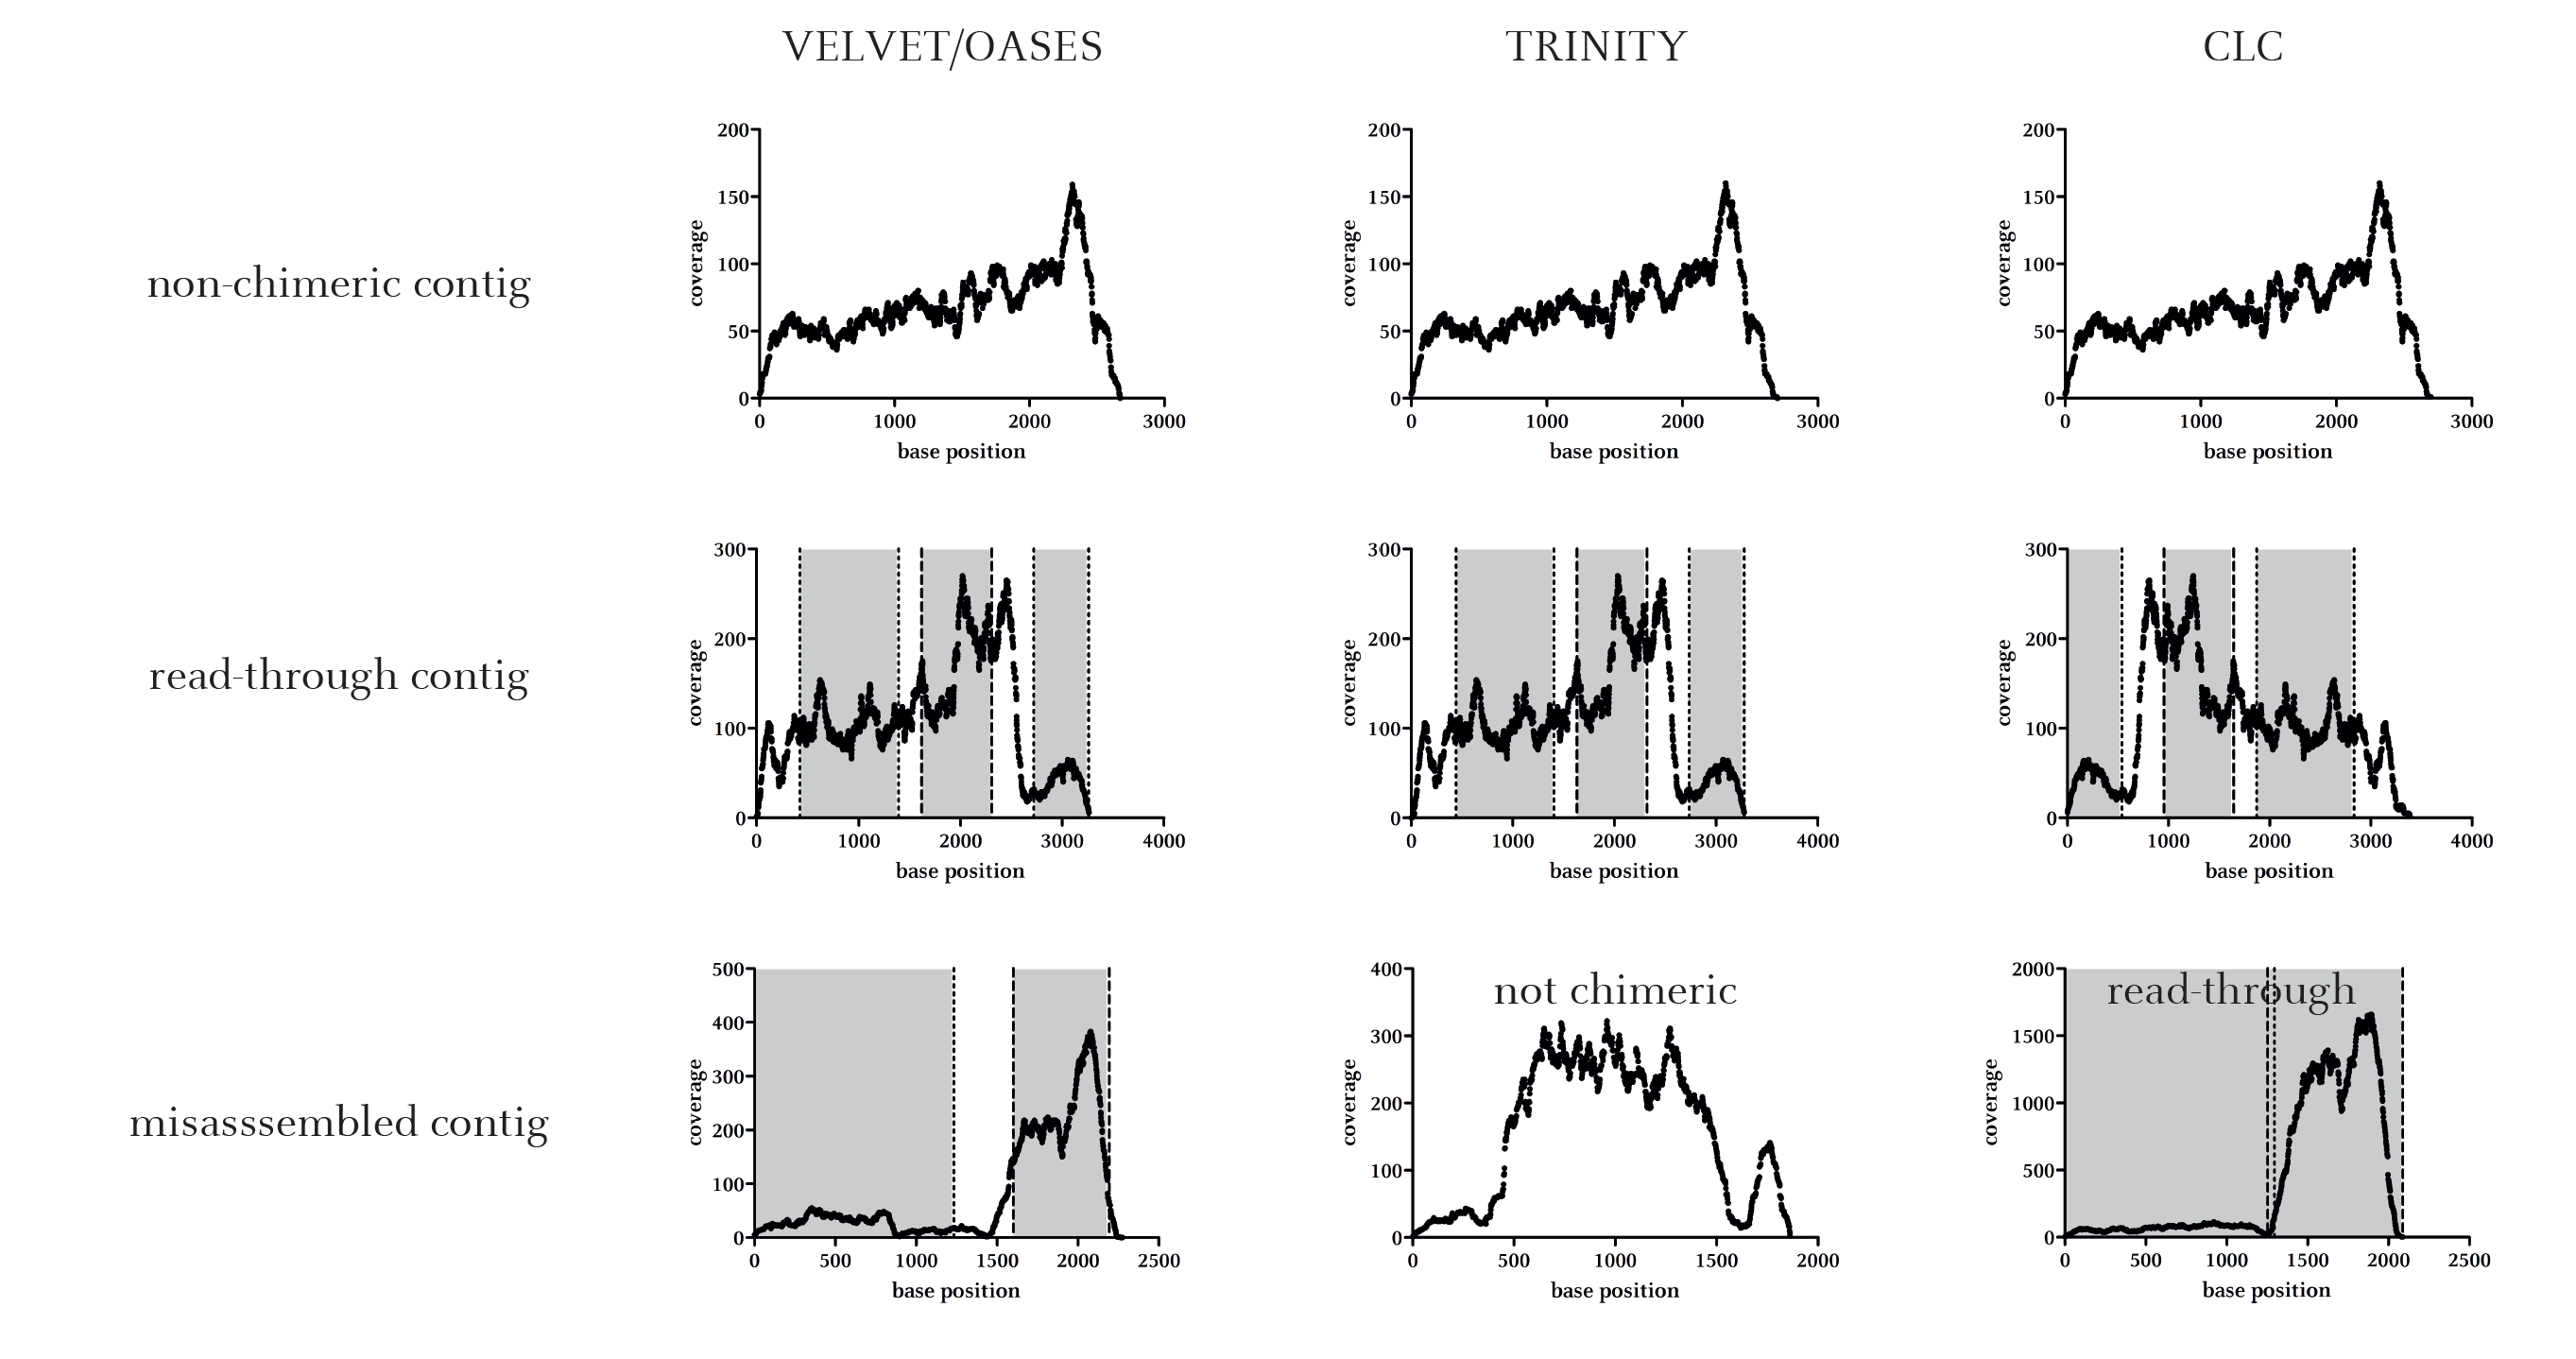
\includegraphics[width=\columnwidth]{images/conclusions_chimeraByExpression}%
					\caption{The read expression across chimeric genes does not reveal the positions of gene fusion marked by dashed lines (determined by mapping to reference genome). (This figure was presented as part of a poster on BioComp2012)}%
					\label{fig:conclusions_chimeraByExpression}%
				\end{figure}
		An approach using expression information to identify the fusion positions did not succeed (figure \ref{fig:conclusions_chimeraByExpression}).
		We tried to identify the fusion sites based on expression coverage of the underlying sequences.
		Unfortunately, we were not able to find a suitable mathematical model to predict these sites reliably.
		As a consequence we were not able to cut fused sequences into their originating transcripts without a priori knowledge about the genome.
		
		% % % One paragraph summary
		Illumina produces a large quantity of short reads with a higher average quality in comparison to 454 sequencing.
		However, \foreignword{de novo} assembly of these is prone to misassemblies, especially invalid fusions of multiple transcripts.
		As there are no means, to detect these in non-model organisms (i.e. without sequenced genome), a different approach is required.
		Assembly of 454 reads results in a much more accurate set of distinct, putative transcripts.
		Hence, it can be used as a sequence reference for sub-cellular localization and for further cloning experiments.
		% % %
		
		%elaborate
		% Answers question on sequencing approach for qualitative aspect

		RNA sequencing is a rapidly evolving technology, so a perfect assembly of the actual transcriptome might be possible with single molecule sequencing techniques.
		However, as of now, these new third generation sequencing technologies are not broadly available.
		For now, most experimentalists continue to use short-read technologies and depend on reliable assembly algorithms.
		Thus, we finally decided to use 454 sequencing to create a reference sequence for \foreignword{in silico} localization.
		Furthermore, to investigate differential gene expression we used deep sequencing technology, Illumina.
		
		
	%Hybrid contigs, Contig and read mapping,
	%Statistics includes papers on Cleome flower and Sulfite oxidase in Arabidopsis
	% Answers question about statistics
	
 \section{Application of NGS to single gene or gene family research}
 % Arabidopsis SO2 and Cleome floral transcriptome
 \subsection{Sulfite oxidase in \species{Arabidopsis}}
 \subsection{Floral timing in \species{Cleome}}
 
 \section{Genome wide transcript analysis}
 \subsection{\species{Dionaea}}
 \begin{itemize}
 	\item Dionaea
 	% Shows that genome wide + exploratory does work.
 \end{itemize}
 \subsection{\species{Megathyrsus maximus}}
% First step confirming \species{D. clandestinum} as suitable C$_3$ comparison partner by biochemical assays.
% Sequencing 
 Expression with a focus on intracellular transport reveals blueprint with coupled transport mechanisms and energy requirements for C$_4$ 4:2.5 similar to C$_3$ 3:2 (ATP:NAD(P)H)
 Traditional approaches (differential expression) not sufficient to understand the whole cycle.
 Function enrichment based on EC and Pfam-Domains provides missing pieces.
 This blueprint supersedes the need for cyclic electron flow and hence dimorphic chloroplasts.
 Cycle can be easily adapted to changing environmental conditions with either increased NAD(P)H production or increased ATP production
 Much simpler than other C$_4$ cycles suggested before.
 C$_4$ has two subtypes NAD-ME+PEP-CK and NADP-ME+PEP-CK with varying ratios of ME:PEP-CK
 Cycle stability achieved through down regulation of pyruvate dehydrogenase in BSC mitochondria and aspartate oxidase in MC cytosol.
 
 Intercellular transport in C$_4$ cycle requires alterations in plasmodesmata.
 An estimate evaluates to 100-fold more transport in C$_4$ compared to C$_3$.
 % current research role of secondary plasmodesmata and callose deposition in C$_4$
 % Answers questions regarding changes between C3 and C4 in multiple aspects (probably need to point that out more specific throughout the text)
 
	\begin{itemize}
		\item PEP-CK/NAD-ME cycle balance
		\item chloroplast transport balancing
		\item ATP for PEP-CK reaction provided through NADPH
		\item Preventing metabolites from leakage to secondary metabolism
		\item EC and Pfam-Domain combinations
		\item intercellular transport
	\end{itemize}
		